\documentclass[aspectratio=169]{beamer}

\usetheme{Madrid}
\usecolortheme{default}

\usepackage{booktabs}
\usepackage{tikz}
\usepackage{hyperref}
\usepackage{lmodern}
\usepackage{graphicx}
\usepackage[table]{xcolor}

% Alternating row colors for tables (automatic)
\definecolor{rowgray}{gray}{0.92}
\rowcolors{2}{rowgray}{white}

% Time formatting
\newcount\myhours
\newcount\myminutes
\myhours=\time \divide\myhours by 60
\myminutes=\time \multiply\myhours by 60 \advance\myminutes by -\myhours
\divide\myhours by 60
\def\mytime{\ifnum\myhours<10 0\fi\the\myhours:\ifnum\myminutes<10 0\fi\the\myminutes}

\title{SpeakUp}
\subtitle{A Systems-Engineering Demonstration}
\author{Bruce Dombrowski}
\date{December 22, 2025}

% Footer with repo link
\setbeamertemplate{footline}{
  \leavevmode%
  \hbox{%
  \begin{beamercolorbox}[wd=.333333\paperwidth,ht=2.25ex,dp=1ex,center]{author in head/foot}%
    \usebeamerfont{author in head/foot}\insertshortauthor
  \end{beamercolorbox}%
  \begin{beamercolorbox}[wd=.333333\paperwidth,ht=2.25ex,dp=1ex,center]{title in head/foot}%
    \usebeamerfont{title in head/foot}\insertshorttitle
  \end{beamercolorbox}%
  \begin{beamercolorbox}[wd=.333333\paperwidth,ht=2.25ex,dp=1ex,right]{date in head/foot}%
    \usebeamerfont{date in head/foot}\insertframenumber{} / \inserttotalframenumber\hspace*{2ex}
  \end{beamercolorbox}}%
  \vskip0pt%
}

\begin{document}

\begin{frame}
\titlepage
\vspace{-1em}
\begin{center}
\small
Repository: \url{https://github.com/brucedombrowski/SpeakUp}\\
\vspace{0.3em}
\footnotesize Generated: \today\ \mytime
\end{center}
\end{frame}

\begin{frame}{About This Document}
\textbf{Purpose:} This briefing is designed for asynchronous review by managers and customers. It can be read independently without a presenter.

\vspace{1em}

\textbf{What SpeakUp Is:}
\begin{itemize}
\item A response to organizational calls for constructive feedback
\item A response to customer requests for process improvement recommendations
\item A demonstration of systems-engineering discipline applied to knowledge work
\item Vendor-neutral at the requirements level---no specific tool is proposed
\item Open source (MIT License)---free to use, modify, and distribute
\end{itemize}

\vspace{1em}

\textbf{Repository:} All artifacts, verification evidence, and this briefing are available at:

\begin{center}
\url{https://github.com/brucedombrowski/SpeakUp}
\end{center}
\end{frame}

\begin{frame}{Problem Statement}
The current operating environment has systemic constraints that limit effectiveness:

\vspace{0.5em}

\begin{table}
\footnotesize
\begin{tabular}{@{}cll@{}}
\toprule
& \textbf{Constraint} & \textbf{Impact} \\
\midrule
1. & Fragmented workflows & Disconnected mobile, desktop, and execution environments \\
2. & Tool accessibility & AI (Artificial Intelligence) unavailable or outside trust boundaries \\
3. & Inbox-centric work & Critical decisions buried in email threads \\
4. & Untracked coordination & Limited traceability and auditability \\
5. & Knowledge attrition & Institutional knowledge lost along with personnel \\
6. & Budget constraints & Reduced investment in tooling, training, modernization \\
7. & Legacy systems & Aging infrastructure facing decommissioning \\
8. & Regulatory burden & Compliance overhead diverts resources from mission work \\
\bottomrule
\end{tabular}
\end{table}
\end{frame}

\begin{frame}{Governing Principles}
\begin{block}{}
\textbf{Resources should be organized to maximize utility.}
\end{block}

\vspace{0.5em}

This is achieved through three guiding principles:

\vspace{0.5em}

\begin{table}
\begin{tabular}{@{}p{3.5cm}p{9.5cm}@{}}
\toprule
\textbf{Principle} & \textbf{Application} \\
\midrule
Transparency & Work is visible to stakeholders; decisions based on shared understanding \\
Inspection & Artifacts and progress reviewed frequently; issues identified early \\
Accountability & Work captured in tracked systems; history preserved for audit \\
\bottomrule
\end{tabular}
\end{table}

\vspace{0.5em}

\footnotesize\textit{Reference: Adapted from Scrum Guide empirical pillars (Schwaber \& Sutherland, 2020)}
\end{frame}

\begin{frame}{Proposed Workflow Model}

\begin{center}
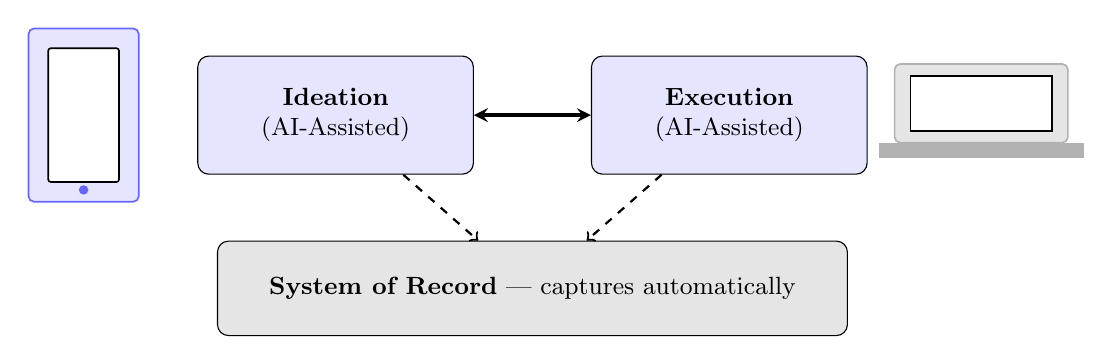
\begin{tikzpicture}[
    workbox/.style={rectangle, draw, rounded corners, minimum width=3.5cm, minimum height=1.5cm, align=center, font=\small, fill=blue!10},
    recordbox/.style={rectangle, draw, rounded corners, minimum width=8cm, minimum height=1.2cm, align=center, font=\small, fill=gray!20},
    arrow/.style={<->, very thick, >=stealth}
]
% Work phases side by side
\node[workbox] (mobile) at (0,0) {\textbf{Ideation}\\(AI-Assisted)};
\node[workbox] (ide) at (5,0) {\textbf{Execution}\\(AI-Assisted)};
% Device callouts added by ChatGPT (GPT-5, Codex CLI) — positioned clear of boxes
\begin{scope}[shift={(-3.2,0)}, line width=0.6pt]
  % Phone icon
  \draw[rounded corners=2pt, fill=blue!10, draw=blue!60] (-0.7,-1.1) rectangle (0.7,1.1);
  \draw[rounded corners=1pt, fill=white] (-0.45,-0.85) rectangle (0.45,0.85);
  \fill[blue!60] (0,-0.95) circle (0.06);
\end{scope}
\begin{scope}[shift={(8.2,0)}, line width=0.6pt]
  % Laptop icon
  \draw[rounded corners=2pt, fill=gray!20, draw=gray!60] (-1.1,-0.35) rectangle (1.1,0.65);
  \draw[fill=white] (-0.9,-0.2) rectangle (0.9,0.5);
  \fill[gray!60] (-1.3,-0.35) rectangle (1.3,-0.55);
\end{scope}

% Bidirectional between phases
\draw[arrow] (mobile) -- (ide);

% System of record below, spanning both
\node[recordbox] (git) at (2.5,-2.2) {\textbf{System of Record} --- captures automatically};

% Dashed arrows showing automatic capture
\draw[->, thick, dashed] (mobile) -- (git);
\draw[->, thick, dashed] (ide) -- (git);
\end{tikzpicture}
\end{center}

\vspace{0.5em}

\begin{columns}
\column{0.5\textwidth}
\textbf{Ideation}
% Updated by ChatGPT (GPT-5, Codex CLI) — clarified ideation bullets
\begin{itemize}
\small
\item Frame objectives, constraints, and risks rapidly
\item Capture rough drafts and decision notes (mobile or desktop)
\item Use text or voice to keep momentum anywhere
\item AI assists synthesis and recommends next steps
\end{itemize}

\column{0.5\textwidth}
\textbf{Execution}
\begin{itemize}
\small
\item Turn drafts into versioned, reviewable artifacts
\item Build inside an IDE with reproducible commands
\item AI assists implementation, refactoring, review, and turnover files
\item Execute inside managed, trusted boundaries
\end{itemize}
\end{columns}

\vspace{0.5em}

\begin{center}
\small Work flows freely between ideation and execution. Recording happens automatically.
\end{center}
\end{frame}

\begin{frame}{Functional Requirements (Solution-Agnostic)}
These requirements define \textit{what} is needed, not \textit{how} to implement it:

\vspace{0.5em}

\begin{table}
\begin{tabular}{@{}llp{8cm}@{}}
\toprule
\textbf{ID} & \textbf{Type} & \textbf{Requirement} \\
\midrule
FR-1 & Mandatory & Mobile ideation capability (smartphone, text/voice input) \\
FR-2 & Mandatory & IDE-centric execution with integrated, replaceable AI assistance \\
FR-3 & Mandatory & Git-based system of record capturing artifacts, history, and rationale \\
FR-4 & Mandatory & Identity and trust boundary alignment (security at identity and device) \\
FR-5 & Recommended & High-signal communication model (email for notification only) \\
\bottomrule
\end{tabular}
\end{table}

\vspace{0.5em}

\small
Full requirements with verification traceability are in the repository: \texttt{README.md}
\end{frame}

\begin{frame}{Security and Compliance}
\textbf{This project is defensible. You can review it without relaxing any rules.}

\vspace{0.5em}

\begin{columns}
\column{0.5\textwidth}
\textbf{What This Repository Contains}
\begin{itemize}
\item No sensitive PII (Personally Identifiable Information)
\item No CUI (Controlled Unclassified Information)
\item No proprietary information
\item No classified information
\item Verified by automated scans producing objective evidence
\end{itemize}

\column{0.5\textwidth}
\textbf{Your Implementation Choices}
\begin{itemize}
\item AI location (cloud, on-prem, local)
\item Repository hosting (GitHub, GitLab, self-hosted)
\item Device policies (BYOD---Bring Your Own Device, managed, air-gapped)
\item Security policies (your existing rules apply)
\end{itemize}
\end{columns}

\vspace{0.5em}

\begin{center}
\small\textit{The workflow pattern is agnostic. Your security posture is your choice.}
\end{center}

\vspace{0.3em}

\small
Verification evidence: \texttt{verification/Compliance-Statement.md}
\end{frame}

\begin{frame}{Value Proposition}
\begin{block}{The Core Point}
\textbf{With the right environment, one person can do the work of an entire team.}
\end{block}

\vspace{0.5em}

\textbf{Example:} This briefing---IDE, AI agent, LaTeX documents, professional PDFs, version control---all produced by one person. The constraint is not capability. It is environment.

\vspace{0.5em}

\begin{table}
\small
\begin{tabular}{@{}p{3.5cm}p{4.5cm}p{5cm}@{}}
\toprule
\textbf{Capability} & \textbf{Current State} & \textbf{Proposed State} \\
\midrule
Work capture & Fragmented, untracked & Structured, version-controlled \\
AI assistance & Outside boundary or unavailable & In-boundary, modular \\
Knowledge preservation & At-risk & Durable artifacts \\
Automation readiness & Limited & Maximized \\
Auditability & Manual effort & Built-in traceability \\
\bottomrule
\end{tabular}
\end{table}
\end{frame}

\begin{frame}{Implementation Approach}
This project demonstrates the pattern by being the pattern:

\vspace{1em}

\begin{itemize}
\item \textbf{Concrete enough to execute}
\begin{itemize}
\item Working repository with all artifacts
\item Defined outputs and verification evidence
\item Reproducible workflow documented in \texttt{artifacts/Workflow-Log.md}
\end{itemize}

\vspace{0.5em}

\item \textbf{Abstract enough to remain vendor and environment neutral}
\begin{itemize}
\item Requirements specify \textit{what}, not \textit{how}
\item Implementation choices documented separately
\item Alternative tools and environments can satisfy same requirements
\end{itemize}

\vspace{0.5em}

\item \textbf{Self-demonstrating}
\begin{itemize}
\item This briefing was created using the proposed workflow
\item Ideation on mobile, execution in IDE, artifacts in Git
\end{itemize}
\end{itemize}

\end{frame}

\begin{frame}{Repository Contents}
All project artifacts are available for review:

\vspace{0.5em}

\begin{table}
\small
\begin{tabular}{@{}ll@{}}
\toprule
\textbf{File} & \textbf{Purpose} \\
\midrule
\texttt{README.md} & Authoritative requirements and project specification \\
\texttt{briefing/SpeakUp-Briefing.pdf} & This document \\
\texttt{verification/Compliance-Statement.md} & Information handling verification evidence \\
\texttt{verification/Requirements-Traceability.md} & Requirements to evidence mapping \\
\texttt{verification/PII-Scan-Results.md} & Automated PII scan test results \\
\texttt{verification/scripts/check-pii.sh} & Automated verification script \\
\texttt{artifacts/Workflow-Log.md} & Execution workflow documentation \\
\bottomrule
\end{tabular}
\end{table}

\vspace{0.5em}

\begin{center}
\url{https://github.com/brucedombrowski/SpeakUp}
\end{center}
\end{frame}

\begin{frame}{Handling Constraints and Blockers}
When a constraint is encountered, the workflow captures it explicitly:

\vspace{0.5em}

\begin{block}{Example: Export Control Constraint}
During BPv7 implementation, NASA TReK was identified as ideal tooling---but is export-controlled (EAR ECCN 9D515.B.5). Rather than stop, the constraint was documented and alternatives evaluated.
\end{block}

\vspace{0.5em}

\begin{table}
\footnotesize
\begin{tabular}{@{}lll@{}}
\toprule
\textbf{Option} & \textbf{Trade-off} & \textbf{Decision} \\
\midrule
NASA TReK & Export controlled (EAR) & Future path \\
NASA JPL ION-DTN & Open source & Selected default \\
Clean-room Python & Full control & Learning/customization \\
\bottomrule
\end{tabular}
\end{table}

\vspace{0.5em}

\textbf{Key Principle:} Constraints become traceable decisions, not invisible blockers.

\textbf{Artifact:} \texttt{artifacts/Decision-Log.md}, \texttt{src/bpv7/simulation/EXPORT\_CONTROL.md}
\end{frame}

\begin{frame}{Requirements Anti-Patterns}
\textbf{Bad specifications cost billions and cause project failures:}

\vspace{0.5em}

\begin{table}
\footnotesize
\begin{tabular}{@{}lll@{}}
\toprule
\textbf{Failure} & \textbf{Cost} & \textbf{Root Cause} \\
\midrule
Mars Climate Orbiter & \$320M & Metric/imperial unit mismatch \\
FBI Virtual Case File & \$170M & Vague requirements, scope creep \\
Ariane 5 Rocket & \$370M & Reused incompatible code \\
\bottomrule
\end{tabular}
\end{table}

\vspace{0.3em}

\begin{table}
\footnotesize
\begin{tabular}{@{}ll@{}}
\toprule
\textbf{Anti-Pattern (FAR 11.104: ``least acceptable'')} & \textbf{Better: Performance Spec} \\
\midrule
``Shall use Microsoft Word'' & ``Shall produce PDF/A archival format'' \\
``Shall be written in Java'' & ``Shall execute on target platform'' \\
``Shall use Oracle database'' & ``Shall persist data with ACID guarantees'' \\
\bottomrule
\end{tabular}
\end{table}

\vspace{0.3em}

\textbf{SpeakUp approach:} LaTeX source (diffable, traceable) $\rightarrow$ PDF output (portable, archival)
\end{frame}

\begin{frame}{Verification Summary}
This project produces verification evidence as first-class artifacts:

\vspace{0.5em}

\begin{table}
\footnotesize
\begin{tabular}{@{}lll@{}}
\toprule
\textbf{Method} & \textbf{Application} & \textbf{NIST\textsuperscript{*} Control} \\
\midrule
Manual Inspection & Document review & --- \\
PII Pattern Scan & Phone, SSN, IP detection & SI-12 \\
Malware Scan & ClamAV detection & SI-3 \\
Secrets Scan & API keys, credentials & SA-11 \\
MAC Address Scan & Hardware identifiers & SC-8 \\
Host Security & OS configuration & CM-6 \\
File Integrity & SHA-256 hashes & SI-7 \\
\bottomrule
\end{tabular}
\end{table}

\vspace{0.2em}
{\scriptsize \textsuperscript{*}NIST: National Institute of Standards and Technology (SP 800-53 Rev 5)}

\vspace{0.3em}

\textbf{Security Attestation:} All automated scans \textbf{PASS}

\textbf{Policy:} Only passing results are published. Vulnerability details are never exposed.
\end{frame}

\begin{frame}{Standards Alignment}
% Added by ChatGPT (GPT-5, Codex CLI) — includes DRAFT watermark for this slide only
\begingroup
\setbeamertemplate{background}{\tikz[remember picture,overlay]{\node[opacity=0.08,scale=6,rotate=45,text=red] at (current page.center) {DRAFT};}}
\textbf{Alignment status (clause-level mapping in work):}

\vspace{0.5em}

\begin{table}
\footnotesize
\begin{tabular}{@{}p{3.4cm}p{6.8cm}p{2cm}@{}}
\toprule
\textbf{Standard} & \textbf{Applicability} & \textbf{Status} \\
\midrule
ISO/IEC/IEEE 15288 & Lifecycle process structure, verification/validation cadence & Aligned \\
ISO/IEC/IEEE 29148 & Requirements quality (shall/should/may, traceability) & Aligned \\
ISO/IEC/IEEE 12207 & Software lifecycle for BPv7 implementation/tests & Aligned \\
ISO/IEC/IEEE 42010 & Architecture rationale and viewpoints (workflow model) & In work \\
ISO/IEC 25010 & Product quality characteristics (security, reliability, maintainability) & In work \\
ISO/IEC 27001 & Security controls baseline; scan attestation supports ISMS evidence & In work \\
\bottomrule
\end{tabular}
\end{table}

\vspace{0.3em}

\footnotesize Clause-level mapping to be added to verification artifacts in the next iteration.
\endgroup
\end{frame}

\begin{frame}{Recommendation}
\textbf{Adopt the SpeakUp workflow model as a pattern for:}

\vspace{1em}

\begin{itemize}
\item Converting thinking into durable, reviewable artifacts
\item Preserving institutional knowledge as personnel transition
\item Enabling automation and reducing manual audit effort
\item Maintaining security and trust boundaries while using AI assistance
\item Improving signal-to-noise in organizational communication
\end{itemize}

\vspace{1em}

\textbf{This pattern is applicable to:}
\begin{itemize}
\item Engineering work
\item Analytical work
\item Knowledge work generally
\end{itemize}
\end{frame}

\begin{frame}{Commit History (Evidence of Work)}
\textbf{15 commits shown (excerpt)} --- full history is 30 commits over ~8 person-hours:

\vspace{0.3em}

\begin{table}
\footnotesize
\begin{tabular}{@{}ll@{}}
\toprule
\textbf{Hash} & \textbf{Commit Message} \\
\midrule
\texttt{9e5aca8} & Update documentation and scan handling \\
\texttt{f1f386e} & Add master build script \\
\texttt{8855611} & Add long-duration DTN test with LOS/AOS \\
\texttt{4090a0a} & Add BPv7 tests and Wireshark demo \\
\texttt{f5d1959} & Update TCPCL to RFC 9174 wire format \\
\texttt{1f3cb42} & Add constraints slide \\
\texttt{cd86850} & Add decision log \\
\texttt{6015094} & Add Docker DTN simulation \\
\texttt{0aecf3c} & Add TCPCL v4 (RFC 9174) \\
\texttt{318800a} & Add BPv7 core (RFC 9171) \\
\texttt{acc6be5} & Add security verification suite \\
\texttt{2b27e68} & Strengthen value proposition \\
\texttt{35a13c7} & Add lifecycle management \\
\texttt{79ac56e} & Add LaTeX briefing deck \\
\texttt{76bd5bc} & Initial commit \\
\bottomrule
\end{tabular}
\end{table}

\vspace{0.3em}

\footnotesize Full commit list via \texttt{git log}. Annotated by ChatGPT (GPT-5, Codex CLI).

\textbf{Key Insight:} 8 hours produced: BPv7 protocol implementation, TCPCL transport, security suite, briefing deck, verification artifacts, and documentation. Each commit captures discrete, traceable work.
\end{frame}

\begin{frame}{Iteration Example: Theme Selection}
\begin{center}
\textbf{Four theme variants produced via rapid iteration:}

\vspace{0.5em}

% Fixed label alignment by using minipages (ChatGPT GPT-5, Codex CLI)
\begin{tabular}{cc}
\begin{minipage}{0.45\linewidth}\centering
\includegraphics[width=0.9\linewidth]{theme-screenshots/theme-madrid.png}\\[-0.2em]
\scriptsize Madrid (Default)
\end{minipage} &
\begin{minipage}{0.45\linewidth}\centering
\includegraphics[width=0.9\linewidth]{theme-screenshots/theme-singapore.png}\\[-0.2em]
\scriptsize Singapore (Seahorse)
\end{minipage} \\\\[1.2em]
\begin{minipage}{0.45\linewidth}\centering
\includegraphics[width=0.9\linewidth]{theme-screenshots/theme-cambridge.png}\\[-0.2em]
\scriptsize CambridgeUS (Dolphin)
\end{minipage} &
\begin{minipage}{0.45\linewidth}\centering
\includegraphics[width=0.9\linewidth]{theme-screenshots/theme-boadilla.png}\\[-0.2em]
\scriptsize Boadilla (Crane)
\end{minipage} \\
\end{tabular}

\vspace{0.5em}

\footnotesize Each variant is a separate commit. Stakeholder selects preferred style. History preserved.
\end{center}
\end{frame}

\begin{frame}{Next Steps}
\begin{enumerate}
\item \textbf{Review this briefing} and the repository contents
\item \textbf{Identify a pilot application area} where the workflow could be applied
\item \textbf{Establish repository and workflow} for the pilot
\item \textbf{Iterate} between ideation and execution phases
\item \textbf{Measure and refine} based on results
\end{enumerate}

\vspace{1.5em}

\begin{center}
\textit{This briefing was produced using the SpeakUp workflow model it describes.}

\vspace{1em}

\textbf{Repository:} \url{https://github.com/brucedombrowski/SpeakUp}

\vspace{0.5em}

\textbf{Contact:} Bruce Dombrowski (Creator)
\end{center}
\end{frame}

\begin{frame}{References}
\footnotesize
\begin{itemize}
\item Schwaber, K. \& Sutherland, J. (2020). \textit{The Scrum Guide}. \url{https://scrumguides.org}
\item NIST SP 800-53 Rev 5. \textit{Security and Privacy Controls for Information Systems}
\item NIST SP 800-171. \textit{Protecting Controlled Unclassified Information}
\item FAR 11.104. \textit{Use of Brand Name or Equal Purchase Descriptions}
\item RFC 9171. \textit{Bundle Protocol Version 7} (CCSDS 734.20-O-1)
\item RFC 9174. \textit{Delay-Tolerant Networking TCP Convergence-Layer Protocol Version 4}
\item RFC 8949. \textit{Concise Binary Object Representation (CBOR)}
\item ISO 32000-2:2020. \textit{PDF/A Archival Format}
% Added by ChatGPT (GPT-5, Codex CLI) — Git reference
\item Git SCM. \textit{Git Reference Manual (git-scm.com/docs)}
\end{itemize}
\end{frame}

\end{document}
